\section{Neural Networks}\label{section:neural-networks}

\begin{wrapfigure}{R}{0.5\textwidth}
% \vspace{-50mm}
    \centering
  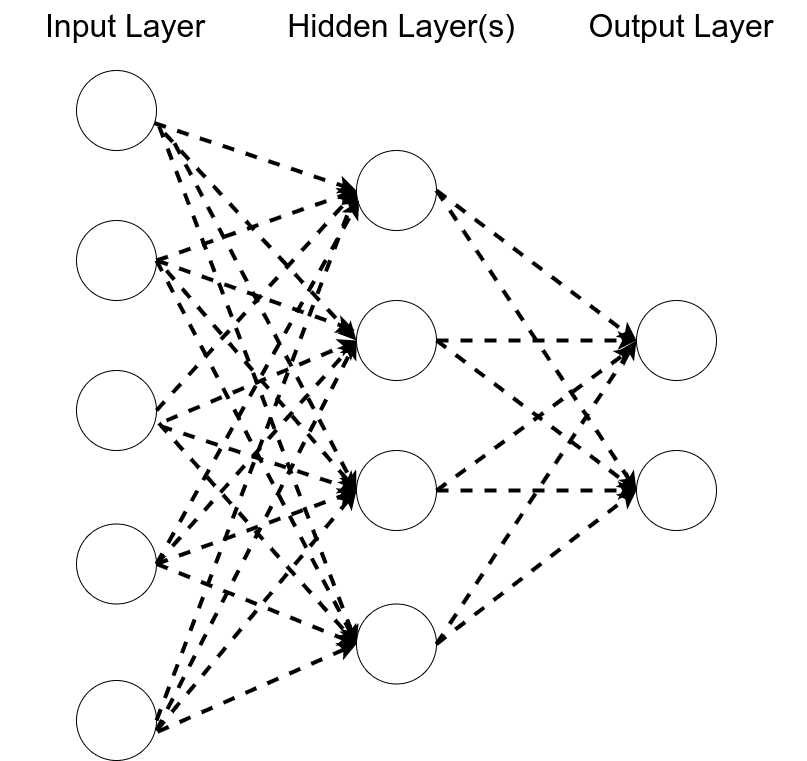
\includegraphics[width=0.45\textwidth]{background/images/neural-network.png}
  \caption{Basic artificial neural network structure.}\label{fig:neural-network}
  \vspace{-16mm}
\end{wrapfigure}

Artificial Neural Networks are systems that are based on the network of neurons of the animal brain \cite{mcculloch1943logical}. These neurons are called \textit{artificial neurons} and are referred to as \textit{nodes}. They are interconnected and organized in \textit{layers} to eventually form a neural network (see Fig. \ref{fig:neural-network}). Each node (represented by a circle) receives the information from the nodes in the previous layer and transmits the new information to the next layer. Input nodes are the exception because they already have the information. New information transmitted by the node is a value from its activation function after receiving all the inputs. The connection between two nodes modifies the output from the lower-layer node before entering the higher-layer node. Most of the networks have an additional bias value for each of the nodes, which can be seen as a regularization parameter. Neural networks have at least three layers: one input layer, one output layer, and at least one hidden layer. The output of the neural network can be defined as:

\begin{equation}\label{eq:forward-pass}
    z^l_j = \sigma \left( \sum_{i}^N(x_i^{l-1} *w_{i,j}^l) + b^l_j \right)
\end{equation}

\newpage

Where:

\begin{itemize}
    \item $l$ is a current layer
    \item $z_j^l$ is an output from the $j$th neuron in layer $l$
    \item $x_i^{l-1}$ is an output from the $i$th neuron on the $l-1$ layer (previous layer)
    \item $w_{i,j}^l$ is a weight for the pair of a current neuron at $j$th position and $i$th neuron from the previous layer
    \item $N$ is a number of neurons in the $l-1$ layer
    \item $b_j^l$ is a bias of $j$th neuron in layer $l$
    \item $\sigma$ is an activation function
\end{itemize}

The goal of a neural network is then finding the value of the weights $w_{ij}^l$ and the biases $b_j^l$ to generate the correct output. These values are optimized in the process called backpropagation.

\subsection{Backpropagation}

Backpropagation is an algorithm that calculates the changes to the weights of the network that are then used to update those weights. The process was first described by Paul Werbos in 1974 \cite{werbos1974beyond}. Even if the name "backpropagation" refers only to gradient computation, it is usually used to describe the whole process of updating the weights. This process consists of three parts. The first part is a feed-forward computation of the input (as defined above), then the error is calculated using the loss function, and lastly, based on the loss function with respect to the weights, the backpropagation computer the gradient used to update the weights.

\vspace{\baselineskip}

After the forward propagation, the error is calculated using a loss function $L(y,\hat{y})$ (where $\hat{y}$ is a predicted output and $y$ is a target output). Usually, the output of the network is a vector $\hat{y} \in \mathbb{R}^n$, and the loss function is a function that translates the difference between $y$ and $y$ into a real number, representing the "cost". One of the simplest loss functions is the Euclidean distance:

\begin{equation}
    L(y,\hat{y}) = \frac{1}{2} || \hat{y} - y  ||^2
\end{equation}

In order to update weights, the gradients have to be calculated with respect to these weights:

\begin{equation}
    \frac{\partial L}{\partial W_l}
\end{equation}

Where $W_l$ is a weight matrix at layer $l$. Computation of that gradient is difficult, but fortunately, the chain rule can be used. It is easier to explain the calculation when the forward function is split into parts (where $\text{CE}$ stands for \textit{Cross-Entropy} loss function defined in equation \ref{eq:cross-entropy}, often used for classification).

\begin{equation}
    z_1 = W_1x + b_1
\end{equation}
\begin{equation}\label{eq:activation-relu}
    h = \text{ReLU}(z_1)
\end{equation}
\begin{equation}
    z_2 = W_2h + b_2
\end{equation}
\begin{equation}
    \hat{y} = \text{sorfmax}(z_2)
\end{equation}
\begin{equation}
    L = \text{CE}(y, \hat{y})
\end{equation}

\begin{equation}\label{eq:cross-entropy}
    \text{CE}(y, \hat{y}) = -(y log(\hat{y}) + (1-y)log(1-\hat{y}))
\end{equation}


Gradient for $W_1$:

\begin{equation}
    \frac{\partial L}{\partial W_1} = \frac{\partial L}{\partial z_2}\frac{\partial z_1}{\partial W_1} = \left( (\hat{y} - y)^Tz_2 \circ sgn(h) \right)^T x^T
\end{equation}

And for $b_1$ :

\begin{equation}
    \frac{\partial L}{\partial w_1} = \frac{\partial L}{\partial z_2}\frac{\partial z_1}{\partial b_1} = \left( (\hat{y} - y)^Tz_2 \circ sgn(h) \right)^T
\end{equation}

Where $sgn$ is a sign function which is a derivative of the ReLU activation function (see eq. \ref{eq:relu-deriv}). With the value of the gradients, weights and biases can be updated.

\subsubsection*{ReLU}

\begin{wrapfigure}{R}{0.30\textwidth}
  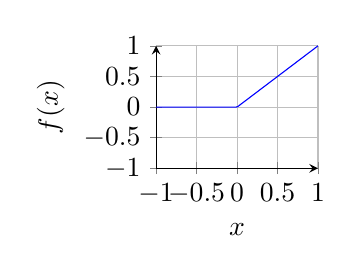
\begin{tikzpicture}
    \begin{axis}[
        axis lines = left,
        xlabel = $x$,
        ylabel = {$f(x)$},
        width=0.3\textwidth,
        ymin = -1,
        ymax = 1,
        grid=both,
        legend pos=north east,
    ]
    %Here the blue parabloa is defined
    \addplot [
        domain=-1:1, 
        samples=100, 
        color=blue,
        ]
        {max(0, x)};
    
    \end{axis}
  \end{tikzpicture}
  \caption{$\text{ReLU}(x)$ where $x \in <-1,1>$}\label{fig:relu-example}
  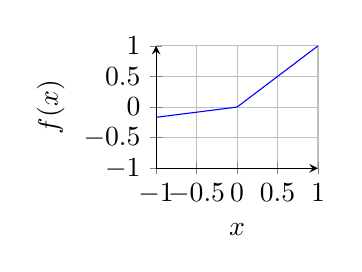
\begin{tikzpicture}
    \begin{axis}[
        axis lines = left,
        xlabel = $x$,
        ylabel = {$f(x)$},
        width=0.3\textwidth,
        ymin = -1,
        ymax = 1,
        grid=both,
        legend pos=north east,
    ]
    %Here the blue parabloa is defined
    \addplot [
        domain=-1:1, 
        samples=100, 
        color=blue,
        ]
        {max(x/6, x)};
    
    \end{axis}
  \end{tikzpicture}
  \caption{$\text{Leaky ReLU}(x)$ where $x \in <-1,1>$}\label{fig:leaky-relu-example}
\end{wrapfigure}

As described in equation \ref{eq:forward-pass} and then later in \ref{eq:activation-relu}, the output is calculated with the use of the activation function. Usually that function is a ReLU function \cite{hahnloser2000digital}. ReLU stands for \textit{Rectified Linear Unit function} and is defined as:

\begin{equation}
    \text{ReLU}(x) = max(x,0)
\end{equation}

and visualized in Figure \ref{fig:relu-example}. Because ReLU returns $0$ every time the value of $x$ is less than $0$, it can deactivate neurons, and therefore create sparser networks. There are two issues with the ReLU function. The first one is that it can create "dead neurons" if all of the inputs of a neuron are less than zero. The second one is that it is not fully differentiable (at the $(0,1)$ point). The first one was solved by Mass et al. \cite{maas2013rectifier} by replacing a zero-valued tail of the ReLU with a slightly negative value $\alpha x$ (where $\alpha$ is a small positive number). Derivative of the ReLU function is defined as follow:

\begin{equation}\label{eq:relu-deriv}
    \text{ReLU}'(x) = \begin{cases} 1 & \text{if } x > 0 \\ 0 & \text{otherwise} \end{cases} = sgn(\text{ReLU}(x))
\end{equation}

\subsection{Convolutional Neural Networks}

Convolutional Neural Network (CNN) \cite{lecun1995convolutional, lecun1989backpropagation} are the type of Neural Networks with at least one convolutional layer. The first convolutional neural networks were LeNet \cite{cnnLecun1998} and AlexNet \cite{krizhevsky2012imagenet}, using only a few convolutional layers. CNNs are assuming that the input data consists of hierarchical patterns which can be used instead of relying on individual features and creating a connection between every single feature and neuron. This approach helps to reduce the number of parameters required by the network.

\subsubsection*{Convolutional Layer}

The convolutional layer uses the idea of filters/kernels with a given size and depth. A layer like that produces the output called a feature map, which is a combination of all the outputs from the kernels. As mentioned, each kernel is defined by the size (which corresponds to its width and height), depths (usually the depth of the input), and additional parameters like padding, stride, or dilatation. The name "convolutional" comes from the mathematical operation of convolution, which is denoted by $f*g$, and the output of that operation is a function that described how one function modifies the other. It can be defined as:

\begin{equation}
    g(m,n) = (h*f)(m,n) = \sum_{u} \sum_{v} h(u,v)f(m-u,n-v)
\end{equation}

Where $f$ is the input image, $h$ is the kernel, $m$ and $n$ are the corresponding row and column in the feature map, and $u$ and $v$ range over all legal subscripts for $h(u,v)$ and $f(m-u,n-v)$ \cite{keller2010convolutions}. An example of the convolution operation for the $m=0, n=3$ is shown in Figure \ref{fig:convolutional operation}.

\begin{figure}[ht]
    \centering
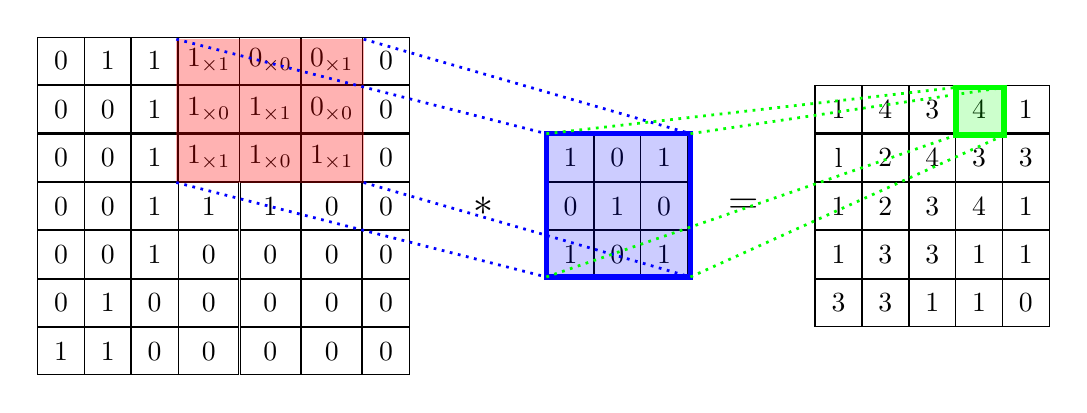
\begin{tikzpicture}[scale=1.0]

  \matrix [nodes=draw,column sep=-0.2mm, minimum size=6mm]
  {
    \node {0}; & \node{1}; & \node {1}; & \node{$1_{\times 1}$}; & \node{$0_{\times 0}$}; 
    & \node{$0_{\times 1}$}; & \node{0}; \\
    \node {0}; & \node{0}; & \node {1}; & \node{$1_{\times 0}$}; & \node{$1_{\times 1}$}; 
    & \node{$0_{\times 0}$}; & \node{0}; \\
    \node {0}; & \node{0}; & \node {1}; & \node{$1_{\times 1}$}; & \node{$1_{\times 0}$}; 
    & \node{$1_{\times 1}$}; & \node{0}; \\
    \node {0}; & \node{0}; & \node {1}; & \node{\, 1 \,}; & \node{\, 1 \, }; 
    & \node{\, 0 \,}; & \node{0}; \\
    \node {0}; & \node{0}; & \node {1}; & \node{\, 0 \, }; & \node{\, 0 \, }; 
    & \node{\, 0 \,}; & \node{0}; \\
    \node {0}; & \node{1}; & \node {0}; & \node{\, 0 \, }; & \node{\, 0 \, }; 
    & \node{\, 0 \,}; & \node{0}; \\
    \node {1}; & \node{1}; & \node {0}; & \node{\, 0 \,}; & \node{\, 0 \, }; 
    & \node{\, 0 \,}; & \node{0}; \\
  };


  % coordinates for coloring filter in array
  \coordinate (A) at (-0.6,0.3);
  \coordinate (B) at (1.78,0.3);
  \coordinate (C) at (1.78,2.12);
  \coordinate (D) at (-0.6,2.12);
  \fill[red, opacity=0.3] (A)--(B)--(C)--(D)--cycle;
  \begin{scope}[shift={(3.3,0)}]
    \node[] at (0,0) {\Large $\ast$};
  \end{scope}[shift={(2.5,0)}]

  \begin{scope}[shift={(5,0)}]

    %\matrix [matrix of math nodes,left delimiter={[},right
    %delimiter={]}]
    \matrix [nodes=draw,column sep=-0.2mm, minimum size=6mm]
    {
      \node{1};  & \node{0};   & \node{1};  \\
      \node{0};  & \node{1};   & \node{0};  \\
      \node{1}; & \node{0}; & \node{1}; \\
    };
    \coordinate (A1) at (-0.9,-0.9);
    \coordinate (B1) at (0.93,-0.9);
    \coordinate (C1) at (0.93,0.92);
    \coordinate (D1) at (-0.9,0.92);
    \fill[blue, opacity=0.2] (A1)--(B1)--(C1)--(D1)--cycle;
    \draw[blue, line width=2] (A1)--(B1)--(C1)--(D1)--cycle;
  \end{scope}

  \draw[dotted, line width=1, color=blue] (A)--(A1);
  \draw[dotted, line width=1, color=blue] (B)--(B1);
  \draw[dotted, line width=1, color=blue] (C)--(C1);
  \draw[dotted, line width=1, color=blue] (D)--(D1);

  \begin{scope}[shift={(6.6,0)}]
    \node[] at (0,0) {\Large $=$};
  \end{scope}[shift={(2.5,0)}]

  \begin{scope}[shift={(9,0)}]

    %\matrix [matrix of math nodes,left delimiter={[},right
    %delimiter={]}]
    \matrix [nodes=draw,column sep=-0.2mm, minimum size=6mm]
    {
      \node{1};  & \node{4};   & \node{3}; & \node{4}; & \node{1};  \\
      \node{l};  & \node{2};   & \node{4}; & \node{3}; & \node{3};  \\
      \node{1}; & \node{2}; & \node{3}; & \node{4} ; & \node{1};  \\
      \node{1}; & \node{3}; & \node{3}; & \node{1} ; & \node{1};  \\
      \node{3}; & \node{3}; & \node{1}; & \node{1} ; & \node{0};  \\
    };
    \coordinate (A2) at (0.3,0.9);
    \coordinate (B2) at (0.91,0.9);
    \coordinate (C2) at (0.91,1.507);
    \coordinate (D2) at (0.3,1.507);
    \fill[green, opacity=0.2] (A2)--(B2)--(C2)--(D2)--cycle;
    \draw[green, line width=2] (A2)--(B2)--(C2)--(D2)--cycle;
  \end{scope}

  \draw[dotted, line width=1, color=green] (A1)--(A2);
  \draw[dotted, line width=1, color=green] (B1)--(B2);
  \draw[dotted, line width=1, color=green] (C1)--(C2);
  \draw[dotted, line width=1, color=green] (D1)--(D2);
\end{tikzpicture}
    \caption{Example of the convolutional operation}
    \label{fig:convolutional operation}
\end{figure}

The standard convolutional layer uses multiple kernels at once, and every one of them has $\text{size} \times \text{size}$ learnable parameters. Putting that in a context where a fully connected neural network requires a weight for every pixel of the input image times the number of neurons in the hidden layer, a convolutional layer is a huge decrease in the total number of parameters. A kernel with a size of $3$ has $9$ learnable parameters. Even with having 50 kernels in the convolutional layer, there are only $450$ learnable parameters in total (for any input image size). For a $32\times32$ image, a fully connected layer with 10 neurons would require $10240$ parameters. It is worth noticing that kernels do not have to be square. The square is computationally efficient, but there were tries to use different shapes \cite{luo2019hexagonal, graham2015sparse, thomas2019kpconv}.

\subsubsection*{Pooling Layer}

CNNs have an additional type of layer called the \textit{Pooling Layer}. There are two types of pooling layers called: \textit{Max Pooling} and \textit{Average Pooling}. Each pooling layer is defined by its size (called the window size), and the result is based only on pixels from that window. The value returned by the max pooling layer is the maximum value from the window. The average pooling layer returns the average from all values from that window.

\begin{figure}[ht]
    \centering
    \begin{subfigure}{.49\textwidth}
        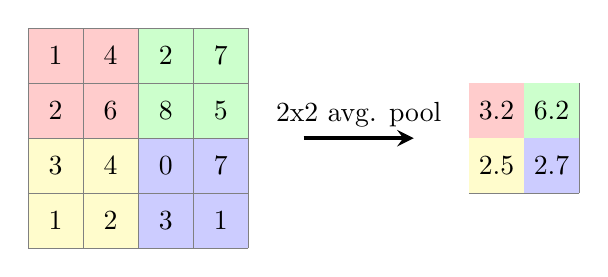
\begin{tikzpicture}[scale=0.7]
        \fill[yellow!20] (0,0) rectangle (2,2);
        \fill[red!20] (0,2) rectangle (2,4);
        \fill[green!20] (2,2) rectangle (4,4);
        \fill[blue!20] (2,2) rectangle (4,0);
        %...
        \draw[gray,very thin] (0,0) grid (4,4);
        \node at (0.5,0.5) {1};
        \node at (1.5,0.5) {2};
        \node at (2.5,0.5) {3};
        \node at (3.5,0.5) {1};
        \node at (0.5,1.5) {3};
        \node at (1.5,1.5) {4};
        \node at (2.5,1.5) {0};
        \node at (3.5,1.5) {7};
        \node at (0.5,2.5) {2};
        \node at (1.5,2.5) {6};
        \node at (2.5,2.5) {8};
        \node at (3.5,2.5) {5};
        \node at (0.5,3.5) {1};
        \node at (1.5,3.5) {4};
        \node at (2.5,3.5) {2};
        \node at (3.5,3.5) {7};
        %...
        \draw[-stealth,ultra thick] (5,2) --node[above] { 2x2 avg. pool} (7,2);
        \draw[gray,very thin] (8,1) grid (10,3);
        \fill[yellow!20] (8,1) rectangle (9,2);
        \fill[red!20] (8,2) rectangle (9,3);
        \fill[green!20] (9,2) rectangle (10,3);
        \fill[blue!20] (9,1) rectangle (10,2);
        \node at (8.5,1.5) {2.5};
        \node at (9.5,1.5) {2.7};
        \node at (8.5,2.5) {3.2};
        \node at (9.5,2.5) {6.2};
        
        \end{tikzpicture}
    \caption{Average Pooling}
    \label{fig:cnn-avg-pooling}
    \end{subfigure}
    \begin{subfigure}{.49\textwidth}
        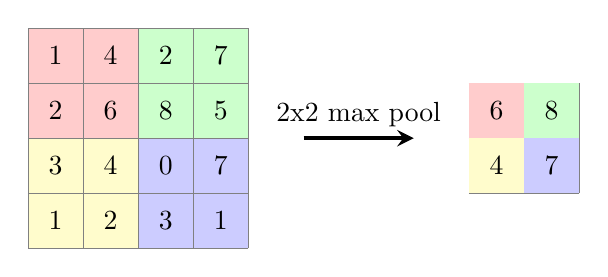
\begin{tikzpicture}[scale=0.7]
        \fill[yellow!20] (0,0) rectangle (2,2);
        \fill[red!20] (0,2) rectangle (2,4);
        \fill[green!20] (2,2) rectangle (4,4);
        \fill[blue!20] (2,2) rectangle (4,0);
        %...
        \draw[gray,very thin] (0,0) grid (4,4);
        \node at (0.5,0.5) {1};
        \node at (1.5,0.5) {2};
        \node at (2.5,0.5) {3};
        \node at (3.5,0.5) {1};
        \node at (0.5,1.5) {3};
        \node at (1.5,1.5) {4};
        \node at (2.5,1.5) {0};
        \node at (3.5,1.5) {7};
        \node at (0.5,2.5) {2};
        \node at (1.5,2.5) {6};
        \node at (2.5,2.5) {8};
        \node at (3.5,2.5) {5};
        \node at (0.5,3.5) {1};
        \node at (1.5,3.5) {4};
        \node at (2.5,3.5) {2};
        \node at (3.5,3.5) {7};
        %...
        \draw[-stealth,ultra thick] (5,2) --node[above] { 2x2 max pool} (7,2);
        \draw[gray,very thin] (8,1) grid (10,3);
        \fill[yellow!20] (8,1) rectangle (9,2);
        \fill[red!20] (8,2) rectangle (9,3);
        \fill[green!20] (9,2) rectangle (10,3);
        \fill[blue!20] (9,1) rectangle (10,2);
        \node at (8.5,1.5) {4};
        \node at (9.5,1.5) {7};
        \node at (8.5,2.5) {6};
        \node at (9.5,2.5) {8};
        
        \end{tikzpicture}
    \caption{Max Pooling}
    \label{fig:cnn-max-pooling}
    \end{subfigure}
    \caption{Example of pooling layers results applied to the same $4 \times 4$ feature map. Colors indicate the area from which the values are pulled to produce the result.}
    \label{fig:cnn-pooling}
\end{figure}